\documentclass{article}
\usepackage{tikz}
\usepackage{pdfpages}
\usepackage{rotating}
\usetikzlibrary{shapes}
\begin{document}

\includepdf[pages={1}]{../assignment_cover_sheet.pdf}

\section*{Question 1}
\subsection*{Insert 1}

\begin{center}
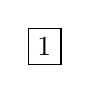
\begin{tikzpicture}
\tikzstyle{bplus}=[rectangle split, rectangle split horizontal,rectangle split ignore empty parts,draw]
\tikzstyle{every node}=[bplus]
\tikzstyle{level 1}=[sibling distance=30mm]
\tikzstyle{level 2}=[sibling distance=10mm]
\node {1}
;\end{tikzpicture}
\end{center}


\subsection*{Insert 79}
\begin{center}
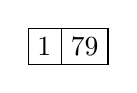
\begin{tikzpicture}
\tikzstyle{bplus}=[rectangle split, rectangle split horizontal,rectangle split ignore empty parts,draw]
\tikzstyle{every node}=[bplus]
\tikzstyle{level 1}=[sibling distance=30mm]
\tikzstyle{level 2}=[sibling distance=10mm]
\node {1 \nodepart{two} 79}
;\end{tikzpicture}
\end{center}

\subsection*{Insert 98}
\begin{center}
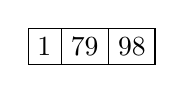
\begin{tikzpicture}
\tikzstyle{bplus}=[rectangle split, rectangle split horizontal,rectangle split ignore empty parts,draw]
\tikzstyle{every node}=[bplus]
\tikzstyle{level 1}=[sibling distance=30mm]
\tikzstyle{level 2}=[sibling distance=10mm]
\node {1 \nodepart{two} 79 \nodepart{three} 98}
;\end{tikzpicture}
\end{center}


\subsection*{Insert 4}
\begin{center}
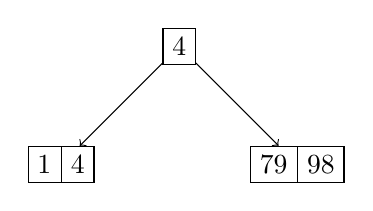
\begin{tikzpicture}
\tikzstyle{bplus}=[rectangle split, rectangle split horizontal,rectangle split ignore empty parts,draw]
\tikzstyle{every node}=[bplus]
\tikzstyle{level 1}=[sibling distance=30mm]
\tikzstyle{level 2}=[sibling distance=10mm]
\node {4} [->]
  child{node {1 \nodepart{two} 4}}
  child{node {79 \nodepart{two} 98}}
;\end{tikzpicture}
\end{center}
Overflow happens resulting in a split.

\subsection*{Insert 69}
\begin{center}
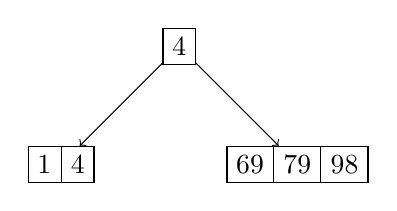
\begin{tikzpicture}
\tikzstyle{bplus}=[rectangle split, rectangle split horizontal,rectangle split ignore empty parts,draw]
\tikzstyle{every node}=[bplus]
\tikzstyle{level 1}=[sibling distance=30mm]
\tikzstyle{level 2}=[sibling distance=10mm]
\node {4} [->]
  child{node {1 \nodepart{two} 4}}
  child{node {69 \nodepart{two} 79 \nodepart{three} 98}}
;\end{tikzpicture}
\end{center}

\subsection*{Insert 2}
\begin{center}
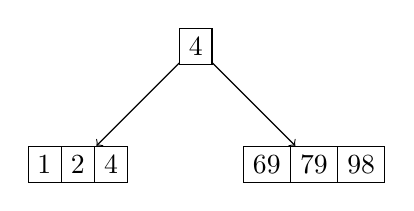
\begin{tikzpicture}
\tikzstyle{bplus}=[rectangle split, rectangle split horizontal,rectangle split ignore empty parts,draw]
\tikzstyle{every node}=[bplus]
\tikzstyle{level 1}=[sibling distance=30mm]
\tikzstyle{level 2}=[sibling distance=10mm]
\node {4} [->]
  child{node {1 \nodepart{two} 2 \nodepart{three} 4}}
  child{node {69 \nodepart{two} 79 \nodepart{three} 98}}
;\end{tikzpicture}
\end{center}

\subsection*{Insert 3}
\begin{center}
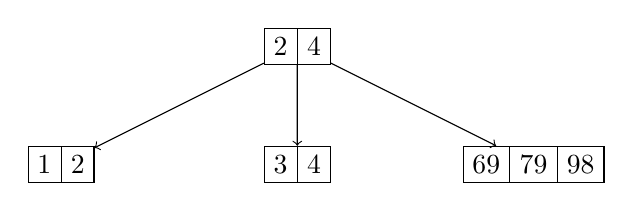
\begin{tikzpicture}
\tikzstyle{bplus}=[rectangle split, rectangle split horizontal,rectangle split ignore empty parts,draw]
\tikzstyle{every node}=[bplus]
\tikzstyle{level 1}=[sibling distance=30mm]
\tikzstyle{level 2}=[sibling distance=10mm]
\node {2 \nodepart {two} 4} [->]
  child{node {1 \nodepart{two} 2}}
  child{node {3 \nodepart{two} 4}}
  child{node {69 \nodepart{two} 79 \nodepart{three} 98}}
;\end{tikzpicture}
\end{center}
Inserting three results in overflow causing a split and sending two up.


\subsection*{Insert 9}
\begin{center}
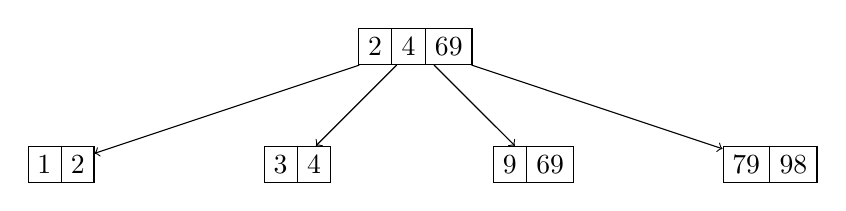
\begin{tikzpicture}
\tikzstyle{bplus}=[rectangle split, rectangle split horizontal,rectangle split ignore empty parts,draw]
\tikzstyle{every node}=[bplus]
\tikzstyle{level 1}=[sibling distance=30mm]
\tikzstyle{level 2}=[sibling distance=10mm]
\node {2 \nodepart {two} 4 \nodepart{three} 69} [->]
  child{node {1 \nodepart{two} 2}}
  child{node {3 \nodepart{two} 4}}
  child{node {9 \nodepart{two} 69}}
  child{node {79 \nodepart{two} 98}}
;\end{tikzpicture}
\end{center}
Inserting nine causes overflow resulting in a split sending sixty nine up.

\subsection*{Insert 8}
\begin{center}
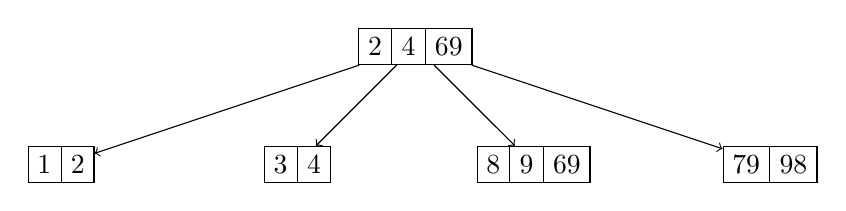
\begin{tikzpicture}
\tikzstyle{bplus}=[rectangle split, rectangle split horizontal,rectangle split ignore empty parts,draw]
\tikzstyle{every node}=[bplus]
\tikzstyle{level 1}=[sibling distance=30mm]
\tikzstyle{level 2}=[sibling distance=10mm]
\node {2 \nodepart {two} 4 \nodepart{three} 69} [->]
  child{node {1 \nodepart{two} 2}}
  child{node {3 \nodepart{two} 4}}
  child{node {8 \nodepart{two} 9 \nodepart{three} 69}}
  child{node {79 \nodepart{two} 98}}
;\end{tikzpicture}
\end{center}

\subsection*{Insert 54}
\begin{center}
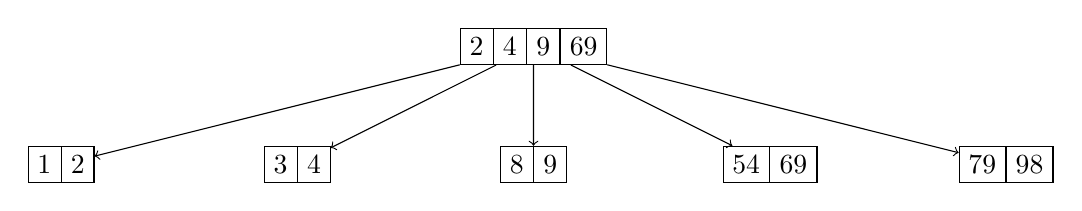
\begin{tikzpicture}
\tikzstyle{bplus}=[rectangle split, rectangle split horizontal,rectangle split ignore empty parts,draw]
\tikzstyle{every node}=[bplus]
\tikzstyle{level 1}=[sibling distance=30mm]
\tikzstyle{level 2}=[sibling distance=10mm]
\node {2 \nodepart {two} 4 \nodepart{three} 9 \nodepart{four} 69} [->]
  child{node {1 \nodepart{two} 2}}
  child{node {3 \nodepart{two} 4}}
  child{node {8 \nodepart{two} 9}}
  child{node {54 \nodepart{two} 69}}
  child{node {79 \nodepart{two} 98}}
;\end{tikzpicture}
\end{center}
Insertion causes overflow resulting in a split.

\subsection*{Insert 92}
\begin{center}
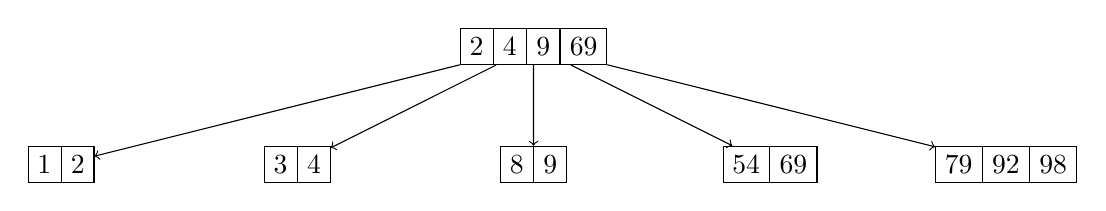
\begin{tikzpicture}
\tikzstyle{bplus}=[rectangle split, rectangle split horizontal,rectangle split ignore empty parts,draw]
\tikzstyle{every node}=[bplus]
\tikzstyle{level 1}=[sibling distance=30mm]
\tikzstyle{level 2}=[sibling distance=10mm]
\node {2 \nodepart {two} 4 \nodepart{three} 9 \nodepart{four} 69} [->]
  child{node {1 \nodepart{two} 2}}
  child{node {3 \nodepart{two} 4}}
  child{node {8 \nodepart{two} 9}}
  child{node {54 \nodepart{two} 69}}
  child{node {79 \nodepart{two} 92 \nodepart{three} 98}}
;\end{tikzpicture}
\end{center}


\subsection*{Insert 97}
\begin{center}
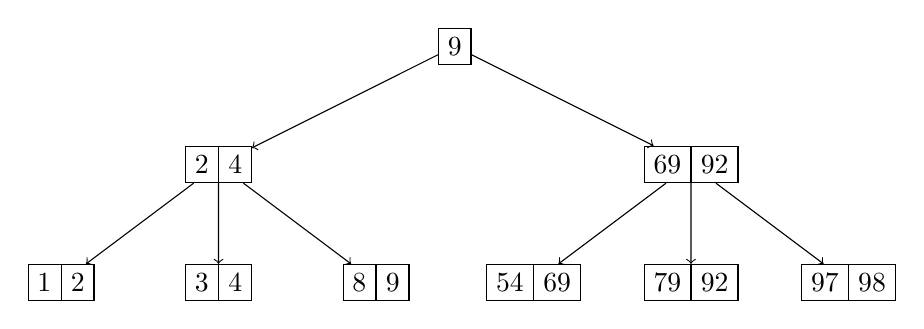
\begin{tikzpicture}
\tikzstyle{bplus}=[rectangle split, rectangle split horizontal,rectangle split ignore empty parts,draw]
\tikzstyle{every node}=[bplus]
\tikzstyle{level 1}=[sibling distance=60mm]
\tikzstyle{level 2}=[sibling distance=20mm]
\tikzstyle{level 3}=[sibling distance=10mm]
\node { 9} [->]
  child{node {2 \nodepart {two} 4 }
    child{node {1 \nodepart{two} 2}}
    child{node {3 \nodepart{two} 4}}
    child{node {8 \nodepart{two} 9}}
  }
  child{node {69 \nodepart{two} 92}
    child{node {54 \nodepart{two} 69}}
    child{node {79 \nodepart{two} 92 }}
    child{node {97 \nodepart{two} 98}}
  }
;\end{tikzpicture}
\end{center}
Insertion causes a split which sends up 92 which causes overflow in the parent node causeing a split and sending 9 up to the root node.


\subsection*{Delete 69}
\begin{center}
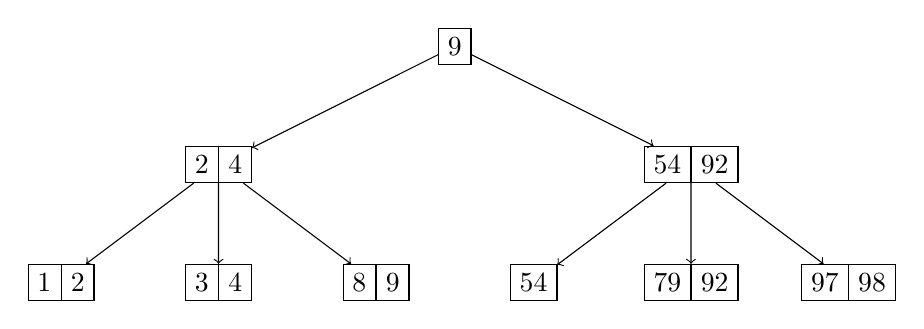
\begin{tikzpicture}
\tikzstyle{bplus}=[rectangle split, rectangle split horizontal,rectangle split ignore empty parts,draw]
\tikzstyle{every node}=[bplus]
\tikzstyle{level 1}=[sibling distance=60mm]
\tikzstyle{level 2}=[sibling distance=20mm]
\tikzstyle{level 3}=[sibling distance=10mm]
\node { 9} [->]
  child{node {2 \nodepart {two} 4 }
    child{node {1 \nodepart{two} 2}}
    child{node {3 \nodepart{two} 4}}
    child{node {8 \nodepart{two} 9}}
  }
  child{node {54 \nodepart{two} 92}
    child{node {54 }}
    child{node {79 \nodepart{two} 92 }}
    child{node {97 \nodepart{two} 98}}
  }
;\end{tikzpicture}
\end{center}

\subsection*{Delete 54}
\begin{center}
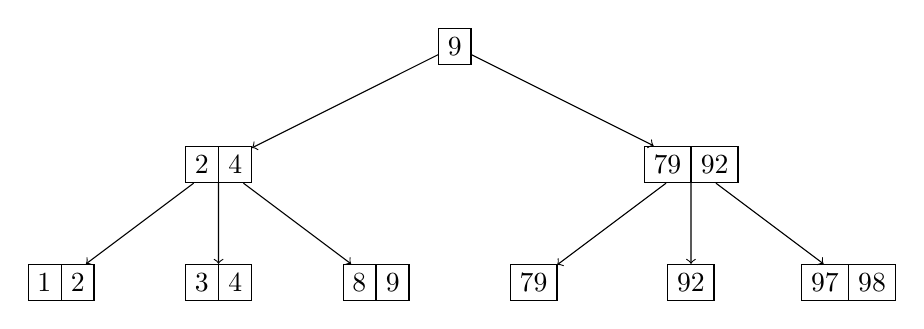
\begin{tikzpicture}
\tikzstyle{bplus}=[rectangle split, rectangle split horizontal,rectangle split ignore empty parts,draw]
\tikzstyle{every node}=[bplus]
\tikzstyle{level 1}=[sibling distance=60mm]
\tikzstyle{level 2}=[sibling distance=20mm]
\tikzstyle{level 3}=[sibling distance=10mm]
\node { 9} [->]
  child{node {2 \nodepart {two} 4 }
    child{node {1 \nodepart{two} 2}}
    child{node {3 \nodepart{two} 4}}
    child{node {8 \nodepart{two} 9}}
  }
  child{node {79 \nodepart{two} 92}
    child{node {79 }}
    child{node {92 }}
    child{node {97 \nodepart{two} 98}}
  }
;\end{tikzpicture}
\end{center}
Merge 79 with empty node.


\subsection*{Delete 92}
\begin{center}
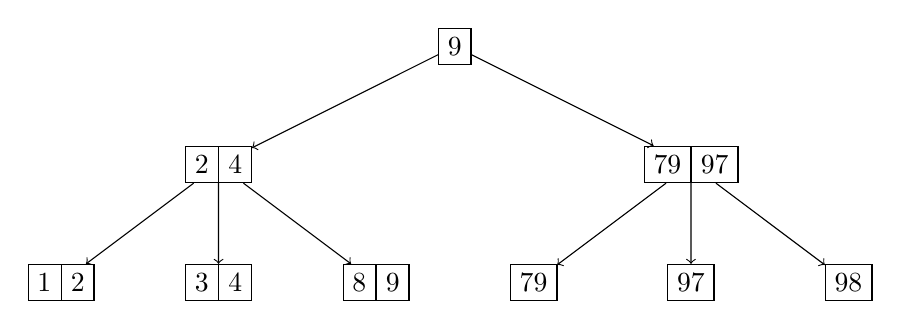
\begin{tikzpicture}
\tikzstyle{bplus}=[rectangle split, rectangle split horizontal,rectangle split ignore empty parts,draw]
\tikzstyle{every node}=[bplus]
\tikzstyle{level 1}=[sibling distance=60mm]
\tikzstyle{level 2}=[sibling distance=20mm]
\tikzstyle{level 3}=[sibling distance=10mm]
\node { 9} [->]
  child{node {2 \nodepart {two} 4 }
    child{node {1 \nodepart{two} 2}}
    child{node {3 \nodepart{two} 4}}
    child{node {8 \nodepart{two} 9}}
  }
  child{node {79 \nodepart{two} 97}
    child{node {79 }}
    child{node {97 }}
    child{node { 98}}
  }
;\end{tikzpicture}
\end{center}
Redistribute 97 from sibling.


\subsection*{Delete 97}
\begin{center}
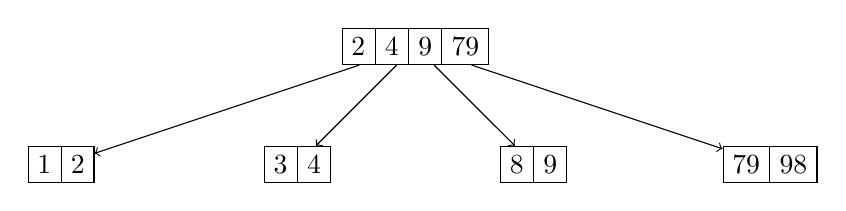
\begin{tikzpicture}
\tikzstyle{bplus}=[rectangle split, rectangle split horizontal,rectangle split ignore empty parts,draw]
\tikzstyle{every node}=[bplus]
\tikzstyle{level 1}=[sibling distance=30mm]
\tikzstyle{level 2}=[sibling distance=10mm]
\node {2 \nodepart {two} 4 \nodepart{three} 9 \nodepart{four} 79} [->]
  child{node {1 \nodepart{two} 2}}
  child{node {3 \nodepart{two} 4}}
  child{node {8 \nodepart{two} 9}}
  child{node {79 \nodepart{two} 98}}
;\end{tikzpicture}
\end{center}
Merge 79 and 98 resulting in underflow of parent node leading to a merge of parents.

\section*{Question 2}
\begin{sidewaysfigure}
\centering
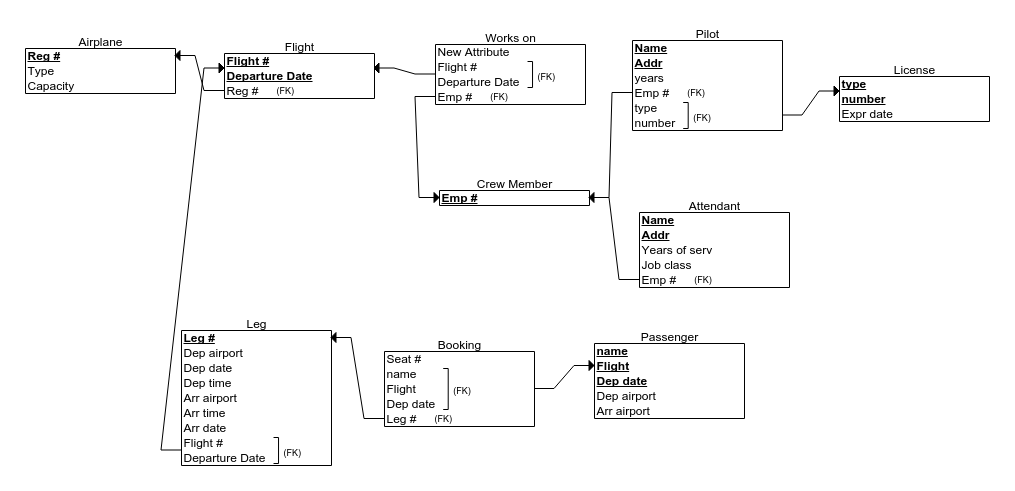
\includegraphics[width=7in]{erd.png}

\end{sidewaysfigure}












\end{document}
